\documentclass{article}
\usepackage[spanish]{babel}
\usepackage[utf8]{inputenc}
\usepackage{amsmath}
\usepackage{amssymb}
\usepackage{graphicx}
\usepackage{listings}
\usepackage{xcolor}
\usepackage{float}
\usepackage{hyperref}
\usepackage{textgreek}
\usepackage{geometry}[margin=1in]

% Configuración para listings (código)
\lstset{
    basicstyle=\ttfamily\small,
    keywordstyle=\color{blue},
    stringstyle=\color{red},
    commentstyle=\color{green!60!black},
    numbers=left,
    numberstyle=\tiny\color{gray},
    stepnumber=1,
    numbersep=5pt,
    backgroundcolor=\color{white},
    showspaces=false,
    showstringspaces=false,
    showtabs=false,
    frame=single,
    rulecolor=\color{black},
    tabsize=2,
    captionpos=b,
    breaklines=true,
    breakatwhitespace=true,
    escapeinside={\%*}{*)}
}

\begin{document}

\begin{titlepage}
  \centering
  
\includegraphics[width=0.25\textwidth]{ITBA_logo.png}\par\vspace{1cm}
  {\textsc{Instituto Tecnológico de Buenos Aires} \par}
    \vspace{1cm}
    {\Large \textsc{Trabajo Práctico 2}\par}
    \vspace{1.5cm}
    {\huge\bfseries Autómatas Celulares\par}
    \vspace{2cm}
    {\Large\itshape Candisano, Gonzalo - 62616\\
	  Neme, Emilio Pablo - 62601\\
	Quian Blanco, Francisco - 63006\par}
    \vfill
    Simulación de Sistemas - 72.25
    \vfill
    \noindent\textbf{Profesores} \\
Parisi, Daniel \\
Patterson, Germán Agustín \\
Salgado Corrado, Ariel Olaf \\
Wiebke, Lucas
\vfill
    {\large Segundo cuatrimestre 2025 - Grupo 12\par}
\end{titlepage}

\section{Introducción}
Este trabajo práctico se enfoca en la simulación de sistemas complejos mediante la implementación y el análisis de un modelo de agente autopropulsado \textit{off-lattice}, basado en los trabajos de Vicsek (y otros) [1] y Baglietto \& Vazquez [2].

\medskip

El objetivo central es estudiar el fenómeno de ordenamiento espontáneo y la transición de fase en un sistema de partículas que interactúan. Para ello, se implementa el modelo clásico de bandadas propuesto en [1], donde cada agente, caracterizado por su posición y velocidad, actualiza su dirección alineándose con la velocidad promedio de sus vecinos dentro de un radio de interacción, añadiendo además un ruido angular de amplitud $\eta$. El grado de orden del sistema se cuantifica mediante el observable de polarización ($v_a$).

\medskip

Posteriormente, se investiga una dinámica de interacción alternativa propuesta en [2], análoga a la de un modelo de votante. En esta variante, la regla de actualización se modifica: en lugar de promediar, cada partícula copia la dirección de velocidad de un único vecino seleccionado al azar dentro de su radio de interacción, sumando también una perturbación de ruido.

\medskip

El presente informe documenta el proceso de simulación, comenzando con la descripción del modelo y su implementación, seguido de los resultados organizados en: a) animaciones de la dinámica del sistema, b) evolución temporal de la polarización, c) curvas de \textit{input} (ruido $\eta$ y densidad $\rho$) vs. \textit{observable} ($v_a$) para ambos modelos, y d) el análisis comparativo de los resultados. Finalmente, se exponen las conclusiones sobre los comportamientos emergentes observados.

\section{Implementación}

\subsection{Descripción del Modelo de Vicsek}
El modelo implementado sigue la formulación de Vicsek (y otros). [1] para partículas autopropulsadas en un espacio bidimensional periódico de tamaño $L \times L$. Cada partícula $i$ está caracterizada por su posición $\vec{x_i}(t) = (x_i(t), y_i(t))$ y su dirección de movimiento $\theta_i(t)$, que evolucionan discretamente en el tiempo según las reglas:

\textbf{a) Actualización de posición:}
\begin{equation}
\vec{x_i}(t + \Delta t) = \vec{x_i}(t) + \vec{v_i}(t) \Delta t
\label{eq:posicion}
\end{equation}

donde $\vec{v_i}(t) = (v \cos \theta_i(t), v \sin \theta_i(t))$ es la velocidad de magnitud constante $v$. La posición se actualiza en cada paso temporal y se aplican condiciones de contorno periódicas.

\textbf{b) Actualización de dirección:}
Se implementaron dos reglas de alineamiento:
\begin{itemize}
\item \textbf{Modelo Clásico (Promedio) [1]:}
\begin{equation}
\theta_i(t + \Delta t) = \langle \theta_j(t) \rangle_{r} + \xi_i(t)
\label{eq:posicion}
\end{equation}
donde $\langle \cdot \rangle_{r}$ denota el promedio angular sobre todas las partículas $j$ (incluyendo a la propia partícula $i$) dentro de un radio de interacción $r$, y $\xi_i(t)$ es un ruido aleatorio uniformemente distribuido en $[-\eta/2, \eta/2]$.

\item \textbf{Modelo de Votante [2]:}
\begin{equation}
\theta_i(t + \Delta t) = \theta_k(t) + \xi_i(t)
\label{eq:posicion}
\end{equation}
donde $k$ es una partícula vecina elegida aleatoriamente (con igual probabilidad) de entre todas las partículas dentro del radio $r$ (incluyéndose a sí misma). $\xi_i(t)$ es el mismo ruido definido en el modelo clásico.
\end{itemize}

\textbf{c) Condiciones de contorno:} Se aplican condiciones periódicas en ambas direcciones para simular un sistema infinito:
\begin{equation}
x_i \leftarrow ((x_i \mod L) + L) \mod L, \quad y_i \leftarrow ((y_i \mod L) + L) \mod L
\label{eq:posicion}
\end{equation}

\subsection{Parámetros del Modelo}
Los principales parámetros del sistema y sus valores típicos o rangos de estudio son:
\begin{itemize}
\item $L$: Tamaño del espacio (longitud del lado del cuadrado). Valor por defecto: \textbf{10}.
\item $N$: Número de partículas. Valor por defecto: \textbf{300}.
\item $v$: Magnitud de la velocidad (constante para todas las partículas). Valor por defecto: \textbf{0.03}.
\item $r$: Radio de interacción. Valor por defecto: \textbf{1.0}.
\item $\eta$: Amplitud del ruido angular. Es la variable de control principal. Valor por defecto: \textbf{0.1}.
\item $\Delta t$: Paso temporal. Valor por defecto: \textbf{1}.
\item $\rho = N/L^2$: Densidad de partículas (parámetro derivado). Variable de estudio secundaria.
\end{itemize}

\subsection{Observable Principal: Polarización}
El grado de orden colectivo del sistema se cuantifica mediante el observable de \textbf{polarización $v_a$}, definido como el módulo del vector velocidad promedio normalizado:
\begin{equation}
v_a(t) = \frac{1}{N v} \left| \sum_{i=1}^{N} \vec{v_i}(t) \right| = \frac{1}{N} \left| \sum_{i=1}^{N} e^{i \theta_i(t)} \right|
\label{eq:posicion}
\end{equation}
donde $v_a \in [0, 1]$. Un valor $v_a \approx 1$ indica un alto grado de alineamiento y la formación de una bandada cohesionada, mientras que $v_a \approx 0$ corresponde a un movimiento desordenado y aleatorio de las partículas.

\subsection{Flujo de la Simulación}
El algoritmo avanza sincrónicamente en pasos de tiempo discretos. En cada iteración o paso $t$:
\begin{enumerate}
\item Para cada partícula, se determina su nuevo ángulo $\theta_i(t + \Delta t)$ según la regla de alineamiento seleccionada (promedio o votante) y el ruido aplicado.
\item Se actualiza la posición de cada partícula utilizando su nueva dirección.
\item Se aplican las condiciones de contorno periódicas a las nuevas posiciones.
\item El estado completo del sistema (x, y, $v_x$, $v_y$ de cada partcula) se escribe en un archivo de texto para su posterior análisis y visualización. Esta separación entre simulación y animación garantiza que la velocidad de visualización no dependa de la velocidad de cálculo del modelo.
\end{enumerate}

\section{Modelo}
El diagrama de clases UML (Figura 1) ilustra la estructura orientada a objetos del código implementado en Java. La simulación consta de:

\begin{itemize}
\item \textbf{Clase \texttt{Main}}: Punto de entrada del programa. Se encarga del parsing de argumentos de línea de comandos, la inicialización del modelo, y la ejecución del loop temporal principal que escribe los estados de las partículas en un archivo de texto.
\item \textbf{Clase \texttt{Vicsek}}: Constituye el núcleo del modelo. Implementa las reglas de actualización de posiciones y direcciones, la detección de vecinos dentro del radio de interacción, y los dos mecanismos de alineamiento (promedio y votante).
\item \textbf{Clase \texttt{Particle}}: Representa el estado de cada agente en el sistema, almacenando su posición (x, y), su dirección de movimiento (theta) y un identificador único (id).
\item \textbf{Clase \texttt{Config}}: Actúa como un contenedor para todos los parámetros de simulación (L, N, v, r, η, etc.), con valores por defecto definidos. Su propósito es organizar y facilitar el paso de estos parámetros a las demás clases.
\end{itemize}

\begin{figure}[H]
\centering
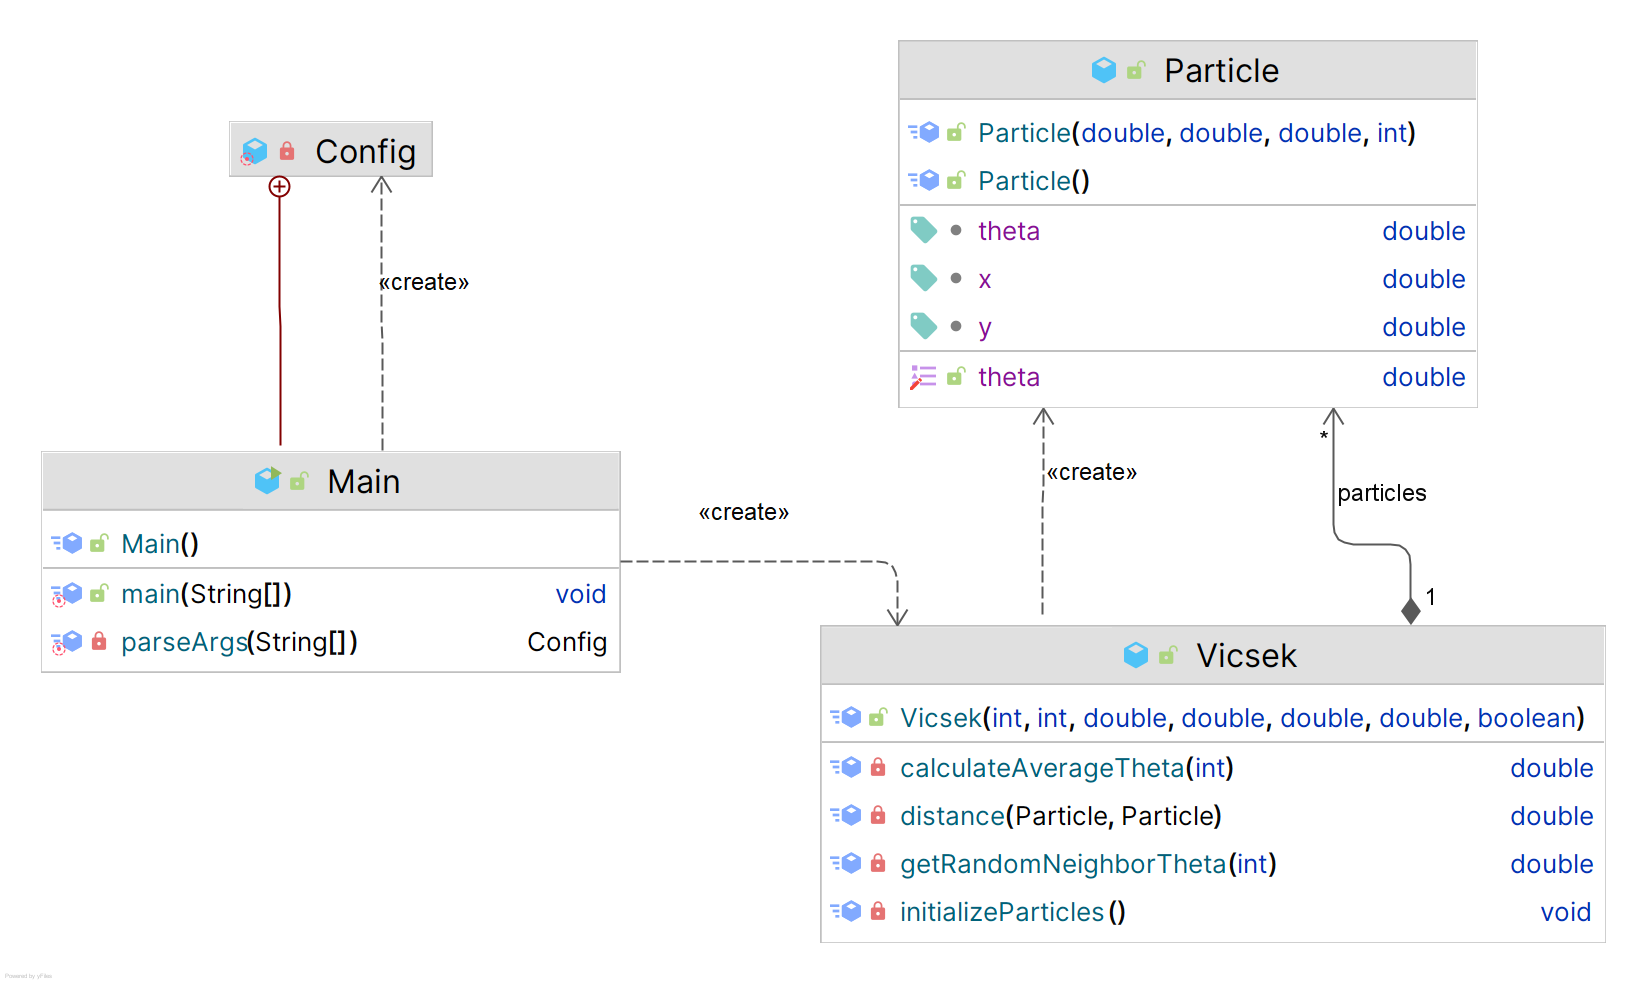
\includegraphics[width=0.9\textwidth]{TP2_UML.png}
\caption{Diagrama de clases UML de la implementación del modelo de Vicsek.}
\label{fig:uml}
\end{figure}

\section{Resultados}

\subsection{Evolución Temporal de la Polarización}
Para caracterizar la dinámica del sistema, se analizó primero la evolución temporal del parámetro de orden $v_a$ en diferentes regímenes de ruido.

\begin{figure}[H]
\centering
\includegraphics[width=0.8\textwidth]{polarizacion_tiempo_sin_ruido.png}
\caption{Evolución temporal de la polarización $v_a(t)$ para $\eta = 0$. Se observa cómo el sistema alcanza rápidamente un estado de orden completo ($v_a \approx 1$) característico del movimiento colectivo coordinado.}
\label{fig:tiempo_sin_ruido}
\end{figure}

\begin{figure}[H]
\centering
\includegraphics[width=0.8\textwidth]{polarizacion_tiempo_con_ruido.png}
\caption{Evolución temporal de la polarización $v_a(t)$ para $\eta = 2.0$. El ruido elevado impide la formación de un estado ordenado, manteniendo el sistema en un régimen desordenado ($v_a \approx 0$) con fluctuaciones características.}
\label{fig:tiempo_con_ruido}
\end{figure}

Las Figuras \ref{fig:tiempo_sin_ruido} y \ref{fig:tiempo_con_ruido} muestran el comportamiento transitorio y estacionario del sistema. Para el análisis cuantitativo, se descartaron los primeros 200 pasos de simulación (régimen transitorio) y se promediaron los valores de $v_a$ sobre 800 pasos adicionales para obtener el valor en estado estacionario.

\subsection{Modelo Clásico (Promedio)}

\subsubsection{Dependencia con el Ruido $\eta$}
\begin{figure}[H]
\centering
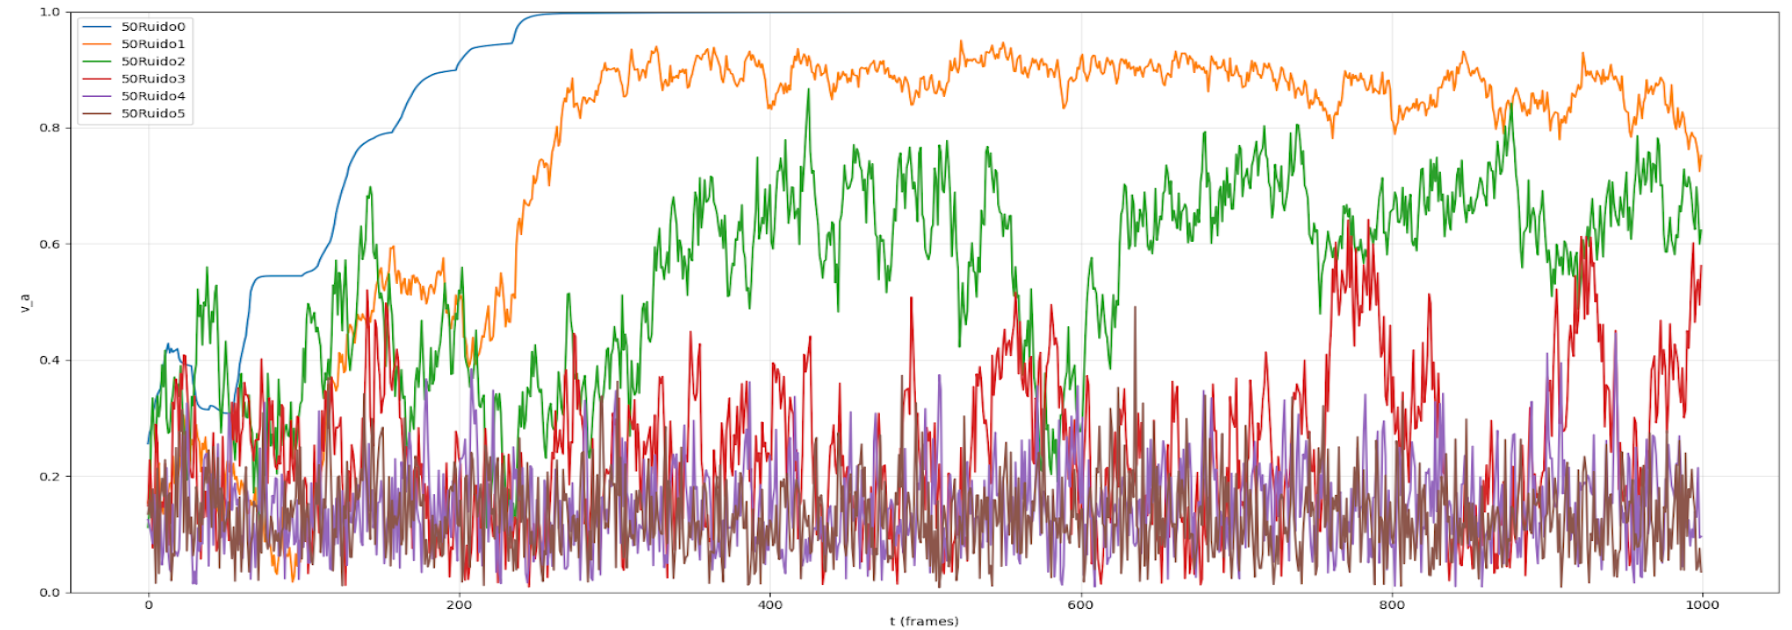
\includegraphics[width=0.8\textwidth]{polarizacion_vs_ruido_promedio.png}
\caption{Polarización $v_a$ en función del ruido $\eta$ para el modelo clásico con $\rho = 3.0$ y $r = 1.0$. Cada punto representa el promedio temporal en estado estacionario, mostrando la transición de fase entre los estados ordenado y desordenado.}
\label{fig:va_vs_eta_promedio}
\end{figure}

\begin{figure}[H]
\centering
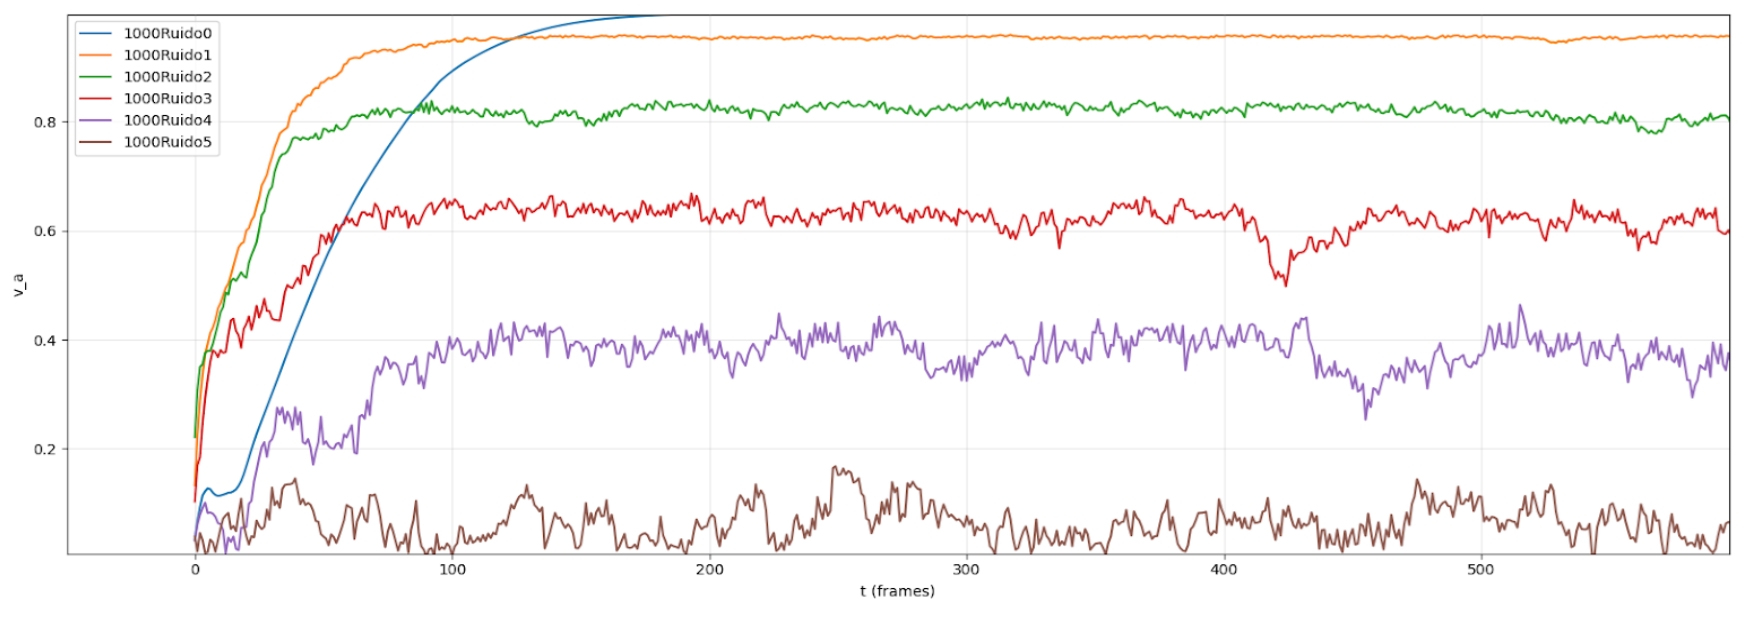
\includegraphics[width=0.8\textwidth]{promedio_polarizacion_ruido_promedio.png}
\caption{Valor promedio de la polarización en estado estacionario en función del ruido $\eta$. Las barras de error representan la desviación estándar temporal. Se observa la criticalidad alrededor de $\eta_c \approx 0.3-0.4$, consistente con los resultados reportados en la literatura [1].}
\label{fig:promedio_va_eta_promedio}
\end{figure}

\subsubsection{Dependencia con la Densidad $\rho$}
\begin{figure}[H]
\centering
\includegraphics[width=0.8\textwidth]{polarizacion_vs_densidad_promedio.png}
\caption{Polarización $v_a$ en función de la densidad $\rho$ para el modelo clásico con $\eta = 0.1$ y $r = 1.0$. La transición a un estado ordenado ocurre a densidades críticas bajas, evidenciando la robustez del fenómeno de flocking.}
\label{fig:va_vs_rho_promedio}
\end{figure}

\begin{figure}[H]
\centering
\includegraphics[width=0.8\textwidth]{promedio_polarizacion_densidad_promedio.png}
\caption{Valor promedio de la polarización en estado estacionario en función de la densidad $\rho$. El sistema muestra una transición suave hacia el estado ordenado a medida que aumenta la densidad de partículas.}
\label{fig:promedio_va_rho_promedio}
\end{figure}

Para el modelo clásico, los resultados muestran una transición de fase bien definida en función del ruido $\eta$ (Figuras \ref{fig:va_vs_eta_promedio} y \ref{fig:promedio_va_eta_promedio}). El valor crítico de ruido $\eta_c \approx 0.3-0.4$ coincide con lo reportado por Vicsek (y otros). [1]. Respecto a la densidad $\rho$, se observa que el sistema alcanza el estado ordenado incluso a densidades relativamente bajas ($\rho > 1.0$), demostrando la eficacia del mecanismo de promediado para establecer orden colectivo.

\subsection{Modelo de Votante}

\subsubsection{Dependencia con el Ruido $\eta$}
\begin{figure}[H]
\centering
\includegraphics[width=0.8\textwidth]{polarizacion_vs_ruido_voter.png}
\caption{Polarización $v_a$ en función del ruido $\eta$ para el modelo de votante con $\rho = 3.0$ y $r = 1.0$. La transición es más abrupta comparada con el modelo clásico.}
\label{fig:va_vs_eta_voter}
\end{figure}

\begin{figure}[H]
\centering
\includegraphics[width=0.8\textwidth]{promedio_polarizacion_ruido_voter.png}
\caption{Valor promedio de la polarización en estado estacionario en función del ruido $\eta$ para el modelo de votante. El sistema muestra una mayor sensibilidad al ruido, con una transición más marcada alrededor de $\eta_c \approx 0.2$.}
\label{fig:promedio_va_eta_voter}
\end{figure}

\subsubsection{Dependencia con la Densidad $\rho$}
\begin{figure}[H]
\centering
\includegraphics[width=0.8\textwidth]{polarizacion_vs_densidad_voter.png}
\caption{Polarización $v_a$ en función de la densidad $\rho$ para el modelo de votante con $\eta = 0.1$ y $r = 1.0$. Se requiere mayor densidad para alcanzar el estado ordenado comparado con el modelo clásico.}
\label{fig:va_vs_rho_voter}
\end{figure}

\begin{figure}[H]
\centering
\includegraphics[width=0.8\textwidth]{promedio_polarizacion_densidad_voter.png}
\caption{Valor promedio de la polarización en estado estacionario en función de la densidad $\rho$ para el modelo de votante. La transición es menos suave y requiere densidades más altas para alcanzar valores elevados de $v_a$.}
\label{fig:promedio_va_rho_voter}
\end{figure}

El modelo de votante (Figuras \ref{fig:va_vs_eta_voter} - \ref{fig:promedio_va_rho_voter}) presenta un comportamiento cualitativamente diferente al modelo clásico. La transición en función del ruido es más abrupta y ocurre a valores críticos más bajos ($\eta_c \approx 0.2$), indicando una mayor fragilidad del estado ordenado frente a perturbaciones. Respecto a la densidad, el modelo de votante requiere valores más altos de $\rho$ para alcanzar el estado ordenado, reflejando la menor eficiencia del mecanismo de copia aleatoria comparado con el promediado colectivo.

\subsection{Análisis Comparativo}
La comparación entre ambos modelos revela diferencias en sus dinámicas colectivas. El modelo clásico, basado en el promedio de sus vecinos, muestra una transición más suave y robusta. Por el contrario, el modelo de votante, al depender de interacciones binarias aleatorias, presenta una transición más abrupta y requiere condiciones más estrictas (menor ruido y mayor densidad) para sostener el estado ordenado.

Estos resultados son consistentes con los reportados por Baglietto \& Vazquez [2], donde se demuestra que las interacciones tipo votante alteran significativamente las propiedades críticas del sistema y la naturaleza de la transición de fase.

\section{Conclusión}

A través de la implementación y análisis computacional de los modelos de Vicsek clásico y de votante, se logró caracterizar y comparar los fenómenos de ordenamiento colectivo en sistemas de partículas autopropulsadas. Los principales hallazgos de este trabajo pueden resumirse en:

\medskip

\textbf{1. Validación del modelo clásico:} Los resultados obtenidos para el modelo de Vicsek clásico reproducen consistentemente los comportamientos reportados en la referencia [1]. Se observó una transición de fase bien definida desde un estado desordenado ($v_a \approx 0$) a un estado ordenado ($v_a \approx 1$) cuando no hay ruido. La dependencia con la densidad mostró que el sistema puede alcanzar el estado ordenado incluso a densidades relativamente bajas ($\rho > 1.0$), demostrando la robustez del mecanismo de promediado colectivo. El ruido claramente afecta a la polarizacion del sistema, haciendo que, con un ruido > 0 la polarización nunca queda estable en 1.

\medskip

\textbf{2. Caracterización del modelo de votante:} El modelo con interacciones tipo votante exhibió un comportamiento cualitativamente diferente. La transición fue más abrupta y ocurrió a valores críticos de ruido más bajos ($\eta_c \approx 0.2$), indicando una mayor sensibilidad a las perturbaciones. Además, requirió densidades significativamente más altas para alcanzar el estado ordenado, reflejando la menor eficiencia del mecanismo de copia aleatoria individual comparado con el promediado colectivo.

\medskip

\textbf{3. Análisis comparativo:} La comparación entre ambos modelos reveló que la naturaleza de las interacciones locales afecta profundamente las propiedades emergentes del sistema. Mientras el modelo clásico muestra una transición suave y robusta característica de sistemas con interacciones cooperativas extendidas, el modelo de votante exhibe una transición más abrupta típica de sistemas con dinámicas de consenso binario.

\medskip

\textbf{4. Implicaciones en modelado de sistemas complejos:} Estos resultados destacan la importancia de la estructura de interacciones en la formación de patrones colectivos en sistemas biológicos y sociales. El hecho de que cambios aparentemente menores en las reglas de interacción (promediado vs. copia aleatoria) produzcan diferencias significativas en el comportamiento macroscópico subraya la necesidad de carefully modelar los mecanismos microscópicos al estudiar fenómenos de emergencia.

\medskip



En síntesis, se demostró exitosamente la implementación computacional de ambos modelos, se caracterizaron sus propiedades críticas y se revelaron las diferencias fundamentales en su comportamiento colectivo, contribuyendo a la comprensión de cómo reglas simples a nivel individual pueden generar comportamientos complejos y diversos a nivel macroscópico.

\begin{thebibliography}{9}
\bibitem{vicsek} 
Vicsek, T., Czirók, A., Ben-Jacob, E., Cohen, I., \& Shochet, O. (1995). Novel type of phase transition in a system of self-driven particles. Physical review letters, 75(6), 1226.

\bibitem{baglietto} 
Baglietto, G., \& Vazquez, F. (2018). Flocking dynamics with voter-like interactions. Journal of Statistical Mechanics: Theory and Experiment, 2018(3), 033403.
\end{thebibliography}

\end{document}